\documentclass[twoside,english,a4paper]{uiofysmaster}
\usepackage{lmodern}
\usepackage[T1]{fontenc}
\usepackage[utf8]{inputenc}

% ----  biblatex ---- %
\usepackage[english]{babel}
\usepackage{csquotes}
\usepackage[backend=biber, sorting=none]{biblatex} % Note that "sorting=none" is NOT the same as leaving the field blank, "sorting=none" means "sorting=citeorder".
\bibliography{JabRef_database,Mendeley_database}

% ---- Code syntax highlighting ---- %
\usepackage[scaled=0.8]{beramono}  % Better monospaced font, nice ~ and ^
% \usepackage[chapter]{minted} % included in uiofysmaster package, to load it before hyperref, to fix \listoflistings
\definecolor{codebg}{rgb}{0.95,0.95,0.95}
\newminted[cppcode]{cpp}{ % can use \newminted{cpp}, gives the same result
    mathescape,
%     frame=lines,
%     framesep=2mm,
    bgcolor = codebg,
    fontsize = \small,
%     fontfamily = courier
} 
% usage: \begin{cppcode}
% use \begin{cppcode*}{<extra options>} if you want to add extra options on the fly

% More options:
% \renewcommand\listingscaption{Program code}
% \renewcommand\listoflistingscaption{List of program codes}

% ----  Draft stuff (remove before final version) ---- %
\usepackage{todonotes}
\usepackage{xcolor}
\newcommand{\orangebox}[1]{
    \fcolorbox{black}{orange}{
        \begin{minipage}{\textwidth}
            #1
        \end{minipage}
    }
}
\usepackage{soulutf8}       % To highlight stuff (when using utf8), using \hl{}. Also has \st{} for strikethrough. Doesn't work that well with equations...
\usepackage{lipsum}

% ---- Images ---- %
\usepackage{graphicx}
\usepackage{svg}            % To include .svg vector graphics directly using \includesvg (will automatically compile/convert the images to .pdf+.pdf_tex using Inkscape). 
                            % NEEDS ``pdflatex --shell-escape'' !!!
\setsvg{                    % conversion options for svg package
    inkscape = inkscape -z -D
}
\usepackage{subcaption}     % The subfigure and subfig packages are deprecated and shouldn't be used any more: 
                            % http://tex.stackexchange.com/questions/144782/subfigure-and-subfig-packages-deprecated
                            % the svg-package originally uses subfig, but replacing subfig with subcaption seems to work

% ---- Other stuff ---- %
% \usepackage{minipage}
\usepackage{commath}        % To correctly typeset differentials \od, \dod, and \tod
\usepackage{fancyvrb}       % Better verbatim, that works inside fcolorbox. Usage: \begin{Verbatim}
\usepackage{cleveref}       % Use \cref{fig:label} instead of \ref{} to get auto ``fig. 1.1a''. \Cref for capitalized.
\usepackage{upgreek}        % Upper case greek letters
\usepackage{bm}             % Bold symbols in math mode
\usepackage{mathtools}      % Mainly for \vdotswithin{=} and \shortvdotswithin{=}
\usepackage{pdfpages}       % To include the frontpage pdf
\usepackage{hyperref}       % Load hyperref package last
% \usepackage{paralist}
\usepackage{relsize}        % To resize stuff - specifically integration signs
\usepackage{exscale}        % To resize integration sign twice

% ---- Custom itemize ---- %
\usepackage{enumitem}       % Better control over enu­mer­ate, item­ize and de­scrip­tion. Su­per­sedes both enu­mer­ate and md­wlist.
\SetEnumitemKey{midsep}{topsep=3pt,partopsep=3pt,parsep=3pt,itemsep=3pt}

% ---- Custom lengths for figures ---- %
% (so we can just use \setlength later)
\newlength{\myfigwidth}
\newlength{\mycaptionwidth}

% ---- Custom commands and symbols ---- %
% ----- Vectors ---- %
% \newcommand{\bvec}[1]{\mathbf{#1}}
\newcommand{\bvec}[1]{\boldsymbol{#1}}    % Using amsmath's boldsymbol
% \newcommand{\bvec}[1]{\bm{#1}}
\newcommand{\rvec}{\bvec{r}}
\newcommand{\vvec}{\bvec{v}}
\newcommand{\avec}{\bvec{a}}
\newcommand{\Fvec}{\bvec{F}}
% ---- Other ---- %
\newcommand{\Ang}{\AA ngstr\"om}
% ---- Other math commands and symbols ---- %
% \newcommand\diff{\mathop{}\!\mathrm{d}}   % Already defined as \dif by commath! But maybe this way is better? Commath uses ``\DeclareMathOperator{\dif}{d \!}''
\newcommand\bigint{\mathop{\mathlarger{\int}}}
\newcommand\biggerint{\mathop{\mathlarger{\mathlarger{\int}}}}

% ---- Fix unicode stuff ---- %
\DeclareUnicodeCharacter{2212}{-}   % Unicode 'MINUS SIGN' (U+2212) that matplotlib uses for minus on axis tick labes

% ---- Formatting ---- %
% skip line instead of indent on new paragraph
\setlength{\parskip}{11pt}
\setlength{\parindent}{0mm}
% make figure text more narrow than textwidth, use small font, and make ``figure'' bold
% ! see alternatives in FYS4180 report
\captionsetup{width=.9\textwidth}
\captionsetup{font=small,labelfont=bf}

\begin{document}

% Front page
\pagenumbering{roman}

\includepdf{frontpage.pdf}
\cleardoublepage

\begin{abstract}
\lipsum
\end{abstract}

\begin{dedication}
  To someone
  \\\vspace{12pt}
  This is a dedication to my cat.
\end{dedication}

\begin{acknowledgements}
  \lipsum
\end{acknowledgements}

\tableofcontents
% \pagenumbering{arabic} -- happens automatically

\listoffigures
\listoftables
\listoflistings


\part{Introduction}
\begin{itemize}
    \item Water confined in nanoporous silica
    \item Characterization of porous silica
    \item 
\end{itemize}


\part{Molecular dynamics}
% To accurately study molecular many-body systems like water confined in nanoporous silica means that we have to consider the quantum mechanical nature of atoms and molecules. To study the motion of atoms using \hl{ab-initio} quantum mechanical calculations, where we have to consider the effect of all electrons, protons and neutrons for all atoms, we have to solve a problem with dimensionality 
% 
% To study water confined in nanoporous silica we use the the method of molecular dynamics simulations. This is a method that use knowledge from the complex quantum mechanical nature of atoms and molecules, to reduce the many-body problems  create simple potentials only depending on the positions \hl{(and velocities?)} of atoms represented as point particles, which we can integrate using Newton's equations of motion. 
% 
% to replacing heavy calculations on the wavefunctions of electrons, protons and neutrons with simple\hl{r} calculations only depending on the positions \hl{(and velocities?)} of point particles representing the positions of the atoms.
% 
% where we approximate the forces between atoms using potentials and parameters from studies and simulations of the underlying quantum mechanical nature of the atoms. This means that we don't have to calculate the exact quantum mechanical interactions between atoms, but instead model the atoms as point particles, with potentials depending on the positions \hl{(and velocities)} of the atoms that give rise to forces. By integrating the forces using Newton's equations of motion
% 
% To do an exact study of the behaviour of atoms and molecules we have to take into account the quantum mechanical workings of such a system. To a silica system we have to consider the that silicon and oxygen consist of  electrons, protons and neutrons of all atoms 

To do an exact study of a many-body atomic system like water confined in nanoporous silica, we have to take into account the quantum mechanical nature of the atoms and molecules in the system. An \hl{average} oxygen molecule consists of 8 electrons, 8 protons and 8 neutrons, all interacting with each other, and each with 3 translational degrees of freedom. This makes doing calculations on something as \hl{``simple''} an electron pretty complex if we want to do it properly. If we want to study a system consisting of more than a couple of oxygen atoms we see that the number of particles and degrees of freedom quickly makes the problem grow to intractable proportions. Since we are mainly interested in the equilibrium and transport properties of the system, we can reduce the problem to something we can handle by using results from underlying quantum mechanical calculations, to develop approximate models of the system. We assume that the many-body system behaves \hl{clasically}\todo{which is an exellent approx. according to Frenkel p 63}, and model all atoms as point particles. From quantum mechanical results we create potentials that approximate the exact forces between the atoms, that only depend on the position \hl{(and velocity?)} of the \hl{atoms/nuclei/point particles}, which are orders of magnitude faster to evaluate compared to calculating the exact forces between the atoms from quantum mechanical principles. We then solve Newton's equations of motion for the system.

To explain how a Molecular Dynamics simulation work we start with a simple example, using one atom type, and a simple model for the force between the atoms. This allows us to get an understanding of the basic concepts used in \hl{MD}. The program actually used for the calculations in the work presented in this thesis uses a very complex potential, and is highly optimized and parallellized for doing calculations on computing clusters on several hundred \hl{CPU's}. But the inner workings of that program \hl{is both a) too much to cover? and b) not necessary to explain?).}

\hl{The idea behind Molecular Dynamics simulations is that we can study the average behaviour of a many-body system by computing the natural time evolution of the system numerically and averaging the quantity of interest over a sufficiently long time.} -- Frenkel p. 15

\chapter{Simulations}
\section{Potential}
\hl{change wording from article supplements}
The interatomic potential we use for for both silica and water consists of 2-body and 3-body terms. The 2-body terms take into account steric repulsion, charge-charge, charge-dipole, and dipole-dipole interactions. The 3-body terms take into account the bending of covalent bonds.
\begin{align*}
    E_\text{tot} = \sum_{i<j} V_{ij}^{(2)}(r_{ij}) + \sum_{i<j<k}V_{ijk}^{(3)}(\rvec_{ij}, \rvec_{ij}).
\end{align*}
The two-body term $V_{ij}^{(2)}$ consists of four terms which take into account steric repulsion, Coulomb, charge-dipole, and van der Waals interaction. The two-body term has the following form
\begin{align*}
    V_{ij}^{(2)} (r) = 
    \underbrace{
        \frac{H_{ij}}{r^{\eta_{ij}}}
    }_{\text{steric repulsion}}
    +~ 
    \underbrace{
        \frac{Z_iZ_j}{r}e^{-r/r_{1\text{s}}}
    }_{\text{Coulomb}}
    ~-~
    \underbrace{
        \frac{D_{ij}}{2r^4}e^{-r/r_{4\text{s}}}
    }_{\text{charge-dipole}}
    ~- 
    \underbrace{
        \frac{w_{ij}}{r^6}
    }_{\text{van der Waals}}
    ,
\end{align*}
where $r$ is the distance between two atoms $i$ and $j$, $H_{ij}$ \hl{controls the steric repulsion}, $Z_i$ is the charge associated with atom $i$, $D_{ij}$ \hl{controls the charge-dipole interaction}, $w_{ij}$ \hl{controls the van der Waals interaction}, and $r_{1\text{s}}$ and $r_{4\text{s}}$ are the screening lengths for the Coulumb and charge-dipole interactions respectively. The three-body term $V_{ijk}^{(3)}$ has the form
\begin{align*}
    &V^{(3)}_{jik}(\rvec_{ij}, \rvec_{ik}) = B_{ijk} \exp\left( \frac{\xi}{r_{ij} - r_0} + \frac{\xi}{r_{ij} - r_0} \right) \frac{\left(\cos\theta_{ijk} - \cos\theta_0\right)^2}{1 + C_{ijk}\left(\cos\theta_{ijk} - \cos\theta_0\right)^2} &(r_{ij}, r_{ik} \leq r_0),
\end{align*}
where $\theta_{ijk}$ is the angle between $\rvec_{ij}$ and $\rvec_{ik}$.

\section{Integration}
% \begin{align*}
%     \rvec(t) = r_n \\
%     \vvec(t) = v_n \\
%     \bvec a(t) = a_n.
% \end{align*}
% \begin{align*}
%     \vvec_{n+1/2} = \vvec_n + \frac{1}{2}\bvec a_n \delta t \\
%     \rvec_{n+1} = \rvec_n + \vvec_{n+\frac{1}{2}}\delta t
% \end{align*}

% \begin{align*}
%     \vvec(t + \Delta t/2) &= \vvec(t) + \frac{1}{2}\bvec a(t) \Delta t \\
%     \rvec(t + \Delta t)   &= \rvec(t) + \vvec(t + \Delta t/2)\Delta t \\
%     \bvec a(t + \Delta t)   &= \frac{1}{m}\Fvec(\rvec(t + \Delta t)) \\
%     \vvec(t + \Delta t)   &= \vvec(t + \Delta t) + \frac{1}{2}\bvec a(t + \Delta t) \Delta t
% \end{align*}

\fcolorbox{black}{orange}{
\begin{minipage}{\textwidth}
{\bf TODO:}
\begin{itemize}
    \item Truncation error Verlet/velociy Verlet
    \item Numerical stability?
    \item Memory?
    \item Self starting, symplectic, reversible
\end{itemize}
\end{minipage}
}

The equations of motion are integrated using the velocity Verlet algorithm:
\begin{align*}
    \rvec(t + \Delta t) &= \rvec(t) + \vvec(t)\Delta t + \frac{\Fvec(t)}{2m}\Delta t^2 \\
    \vvec(t + \Delta t) &= \vvec(t) + \frac{\Fvec(t + \Delta t) + \Fvec(t)}{2m}\Delta t
\end{align*}


\subsection{Derivation of Verlet algorithm}
\todo{why do we use velocity Verlet}
The Verlet algorithm\cite{verlet1967computer} is a simple method for integrating second order differential equations of the form 
\begin{align*}
    \dod[2]{\rvec(t)}{t} = \Fvec\big[\rvec(t), t\big] = \Fvec(t).
\end{align*}
We first let
\begin{align*}
    \dod{\rvec(t)}{t} &= \vvec(t),
\end{align*}
and
\begin{align*}
    \dod{\vvec(t)}{t} &= \frac{\Fvec(t)}{m}.
\end{align*}

We then do a Taylor expansion of $\rvec(t \pm \Delta t)$ around time $t$
\begin{align}
    \rvec(t + \Delta t) &= \rvec(t) + \vvec(t)\Delta t + \frac{\Fvec(t)}{m}\frac{\Delta t^2}{2} + \dod[3]{\rvec(0)}{t}\frac{\Delta t^3}{6} + \mathcal{O}(\Delta t^4), \label{eq:verlet_plus}\\
    \rvec(t - \Delta t) &= \rvec(t) - \vvec(t)\Delta t + \frac{\Fvec(t)}{m}\frac{\Delta t^2}{2} - \dod[3]{\rvec(0)}{t}\frac{\Delta t^3}{6} + \mathcal{O}(\Delta t^4).\label{eq:verlet_minus}
\end{align}
By summing these two equations we get
\begin{align*}
    \rvec(t + \Delta t) + \rvec(t - \Delta t) = 2\rvec(t) + \frac{\Fvec(t)}{m}\Delta t^2 + \mathcal{O}(\Delta t^4),
\end{align*}
which by rearranging can be written as
\begin{align*}
    \rvec(t + \Delta t) \approx 2\rvec(t) - \rvec(t - \Delta t) + \frac{\Fvec(t)}{m}\Delta t^2,
\end{align*}
Which is the equation used to update the positions in the regular Verlet algorithm. We see that the estimate of the new position contains an truncation error for one timestep $\Delta t$ of the order $\mathcal{O}(\Delta t^4)$.

The Verlet algorithm does not use the velocity to compute the new position, but we can find an estimate of the velocity by taking the difference between equations \eqref{eq:verlet_plus} and \eqref{eq:verlet_minus}
\begin{align*}
    \rvec(t + \Delta t) - \rvec(t - \Delta t) = 2\vvec(t)\Delta t + \mathcal{O}(\Delta t^3),
\end{align*}
which by rearranging can be written as
\begin{align*}
    \vvec(t) = \frac{\rvec(t + \Delta t) - \rvec(t - \Delta t)}{2\Delta t} + \mathcal{O}(\Delta t^2).
\end{align*}
We see that this estimate of the velocity has a truncation error of the order $\mathcal{O}(\Delta t^2)$, compared to the error in the position $\mathcal{O}(\Delta t^4)$.
\todo{Something about lower precision}

A modification of the Verlet algorithm usually called the velocity Verlet algorithm\cite{swope1982computer} \todo{something about why velocity Verlet is good} can be derived in a similar way. We have the same Taylor expansion of $\rvec(t+\Delta t)$ around $t$ as before
\begin{align}
    \rvec(t + \Delta t) &= \rvec(t) + \vvec(t)\Delta t + \frac{\Fvec(t)}{m}\frac{\Delta t^2}{2} + \mathcal{O}(\Delta t^3), \label{eq:position_taylor}
\end{align}
and now we also expand $\vvec(t + \Delta t)$ around $t$
\begin{align}
    \vvec(t + \Delta t) 
%     &= \vvec(t) + \dod{\vvec(t)}{t}\Delta t + \dod[2]{\vvec(t)}{t}\frac{\Delta t^2}{t} + \mathcal{O}(\Delta t^3) \\
    &= \vvec(t) + \frac{\Fvec(t)}{m}\Delta t + \dod[2]{\vvec(t)}{t}\frac{\Delta t^2}{2} + \mathcal{O}(\Delta t^3).\label{eq:velocity_taylor}
\end{align}
We now need an expression for $\od[2]{\vvec(t)}{t}$, which can be found by a Taylor expansion of $\od{\vvec(t+\Delta t)}{t}$
\begin{align*}
    \dod{\vvec(t+\Delta t)}{t} = \dod{\vvec(t)}{t} + \dod[2]{\vvec(t)}{t}\Delta t + \mathcal{O}(\Delta t^2),
\end{align*}
which by rearranging and multiplying with $\frac{\Delta t}{2}$ gives
\begin{align*}
    \dod[2]{\vvec}{t}\frac{\Delta t^2}{2} 
    &= \frac{\Delta t}{2}\left( \dod{\vvec(t+\Delta t)}{t} - \dod{\vvec(t)}{t}\right) + \mathcal{O}(\Delta t^3) \\
    &= \frac{\Fvec(t + \Delta t) - \Fvec(t)}{m} \frac{\Delta t}{2} + \mathcal{O}(\Delta t^3).
\end{align*}
Inserting this into Eq. \eqref{eq:velocity_taylor} we get
\begin{align*}
    \vvec(t + \Delta t) 
    &= \vvec(t) + \frac{\Fvec(t)}{m}\Delta t + \frac{\Fvec(t + \Delta t) - \Fvec(t)}{m} \frac{\Delta t}{2} + \mathcal{O}(\Delta t^3) \\
    &= \vvec(t) + \frac{\Fvec(t + \Delta t) + \Fvec(t)}{m} \frac{\Delta t}{2} + \mathcal{O}(\Delta t^3).
\end{align*}
So the total velocity Verlet algorithm with truncation of the higher-order terms is
\begin{align}
    \rvec(t + \Delta t) &= \rvec(t) + \vvec(t)\Delta t + \frac{\Fvec(t)}{m}\frac{\Delta t^2}{2}, \label{eq:velocity_verlet_position}\\
    \vvec(t + \Delta t) &= \vvec(t) + \frac{\Fvec(t + \Delta t) + \Fvec(t)}{m} \frac{\Delta t}{2}\label{eq:velocity_verlet_velocity},
\end{align}
with the truncation error for one timestep $\Delta t$ being of the order $\mathcal{O}(\Delta t^3)$ for both the position and the velocity. 

The algorithm is usually rewritten in the following way, to optimize the implementation on a computer. We see that
\begin{align}
    \vvec(t+\Delta t) = \vvec(t + \tfrac{1}{2}\Delta t) + \frac{\Fvec(t + \Delta t)}{m}\frac{\Delta t}{2},\label{eq:verlet_velocity_with_halfstep}
\end{align}
where
\begin{align}
    \vvec(t + \tfrac{1}{2}\Delta t) = \vvec(t) + \frac{\Fvec(t)}{m}\frac{\Delta t}{2}.\label{eq:verlet_halfstep}
\end{align}
\todo[inline]{(not really true??? compared to $\vvec(t+\Delta t/2)$ with equation \eqref{eq:velocity_verlet_velocity})} Which gives us the usual way of implementing the algorithm\cite{allen1989computer}, as follows
\begin{itemize}
    \item Calculate the new positions at $t + \Delta t$ using Eq. \eqref{eq:velocity_verlet_position} \hl{(repeated here)}
    \begin{align*}
        \rvec(t + \Delta t) &= \rvec(t) + \vvec(t)\Delta t + \frac{\Fvec(t)}{m}\frac{\Delta t^2}{2}.
    \end{align*}
    \item Calculate the velocities at $t+\tfrac{1}{2}\Delta t$ using Eq. \eqref{eq:verlet_halfstep} \hl{(repeated here)}
    \begin{align*}
        \vvec(t + \tfrac{1}{2}\Delta t) = \vvec(t) + \frac{\Fvec(t)}{m}\frac{\Delta t}{2}.
    \end{align*}
    \item Calculate the new forces $\Fvec(t+\Delta t)$.
    \item Calculate the new velocities at $t+\Delta t$ using Eq. \eqref{eq:verlet_velocity_with_halfstep} \hl{(repeated here)}
    \begin{align*}
        \vvec(t+\Delta t) = \vvec(t + \tfrac{1}{2}\Delta t) + \frac{\Fvec(t + \Delta t)}{m}\frac{\Delta t}{2}.
    \end{align*}
\end{itemize}
This implementation minimizes the memory needs, as we only need to store one copy of $\rvec$, $\vvec$ and $\Fvec$ at all times. Pseudocode: \todo{do we want/need this?}
\begin{verbatim}
    r += v*dt + F*dt*dt/(2*m);
    v += F*dt/(2*m);
    F = calculate_forces(r, v);
    v += F*dt/(2*m);
\end{verbatim}


% The velocity Verlet algorithm can be implemented as follows\cite{allen1989computer}
% \begin{samepage}
% \begin{itemize}
%     \item Calculate the new positions at $t + \Delta t$ using Eq. \eqref{eq:velocity_verlet_position}.
%     \item Calculate the velocities at $t + \frac{1}{2}\Delta t$ using
%     \begin{align*}
%         \vvec(t + \tfrac{1}{2}\Delta t) = \vvec(t) + \frac{\Fvec(t)}{m}\frac{\Delta t}{2}.
%     \end{align*}
%     \item Calculate the new forces $\Fvec(t + \Delta t)$.
%     \item Finally, calculate the new velocities at $t + \Delta t$ using
%     \begin{align*}
%         \vvec(t + \Delta t) = \vvec(t + \tfrac{1}{2}\Delta t) + \frac{\Fvec(t + \Delta t)}{m}\frac{\Delta t}{2}
%     \end{align*}
% \end{itemize}
% \end{samepage}
% But 
% This implementation uses $9N$ units of memory, 

\subsection{Global error in the Verlet algorithm}
\fcolorbox{black}{orange}{
\begin{minipage}{\textwidth}
Sources:
\begin{itemize}
    \item \url{http://math.stackexchange.com/questions/668707/verlet-method-global-error}
    \item \url{http://www.saylor.org/site/wp-content/uploads/2011/06/MA221-6.1.pdf} (same as Wikipedia)
\end{itemize}

    The global error in position can be derived from the local error for one timestep $\Delta t$. We see from Eq. \eqref{eq:position_taylor} that
    \begin{align*}
        \text{error}\big(\rvec(t+\Delta t)\big) = \mathcal{O}(\Delta t^3).
    \end{align*}
    The error for two timesteps is
    \begin{align*}
        \rvec(t+2\Delta t) 
        &= \rvec(t+\Delta t) + \vvec(t+\Delta t)\Delta t + \frac{\Fvec(t+\Delta t)}{m}\frac{\Delta t^2}{2} + \mathcal{O}(\Delta t^3),
        &= \rvec()
    \end{align*}
    which gives
    \begin{align*}
        \text{error}\big(\rvec(t+2\Delta t)\big) = 
    \end{align*}
\end{minipage}
}

\section{Ensemble, observables etc.}
\section{Initialization}
\section{Passivation}
\begin{itemize}
    \item Tetrahedra
    \item Neighbor lists -- see base\_code/passivate\_using\_tetrahedra/passivator.cpp near line 700
    \begin{itemize}
        \item Create list of atoms in each voxel
        \item Create neighbor lists for each atom by looping through neighbor voxels for each atoms
    \end{itemize}
    \item Count number of neighbors of different types -- find number of missing neighbors, Si - 4 Oxygen, Oxygen 2 Si
    \item Insert OH on Si with missing O neighbors, insert H on Oxygen with missing Si neighbors
    \begin{itemize}
        \item Insert O/H at good angles
    \end{itemize}
    \item Improvement: find the atoms near surface using voxels, only passivate those atoms
\end{itemize}

\section{Injecting water}
\begin{itemize}
    \item Voxelize system -- size depends on wanted density
    \item Mark all voxels within distance from other atoms as occupied
    \item Fill other voxels with H2O with random O-H orientation, but correct angle
    \item Improvement: Use one voxel size in the beginning (to avoid one-voxel pores), and then use a smaller voxel size when injecting water
\end{itemize}
    
\chapter{Fractures}

\begin{figure}[h!]
    \centering
    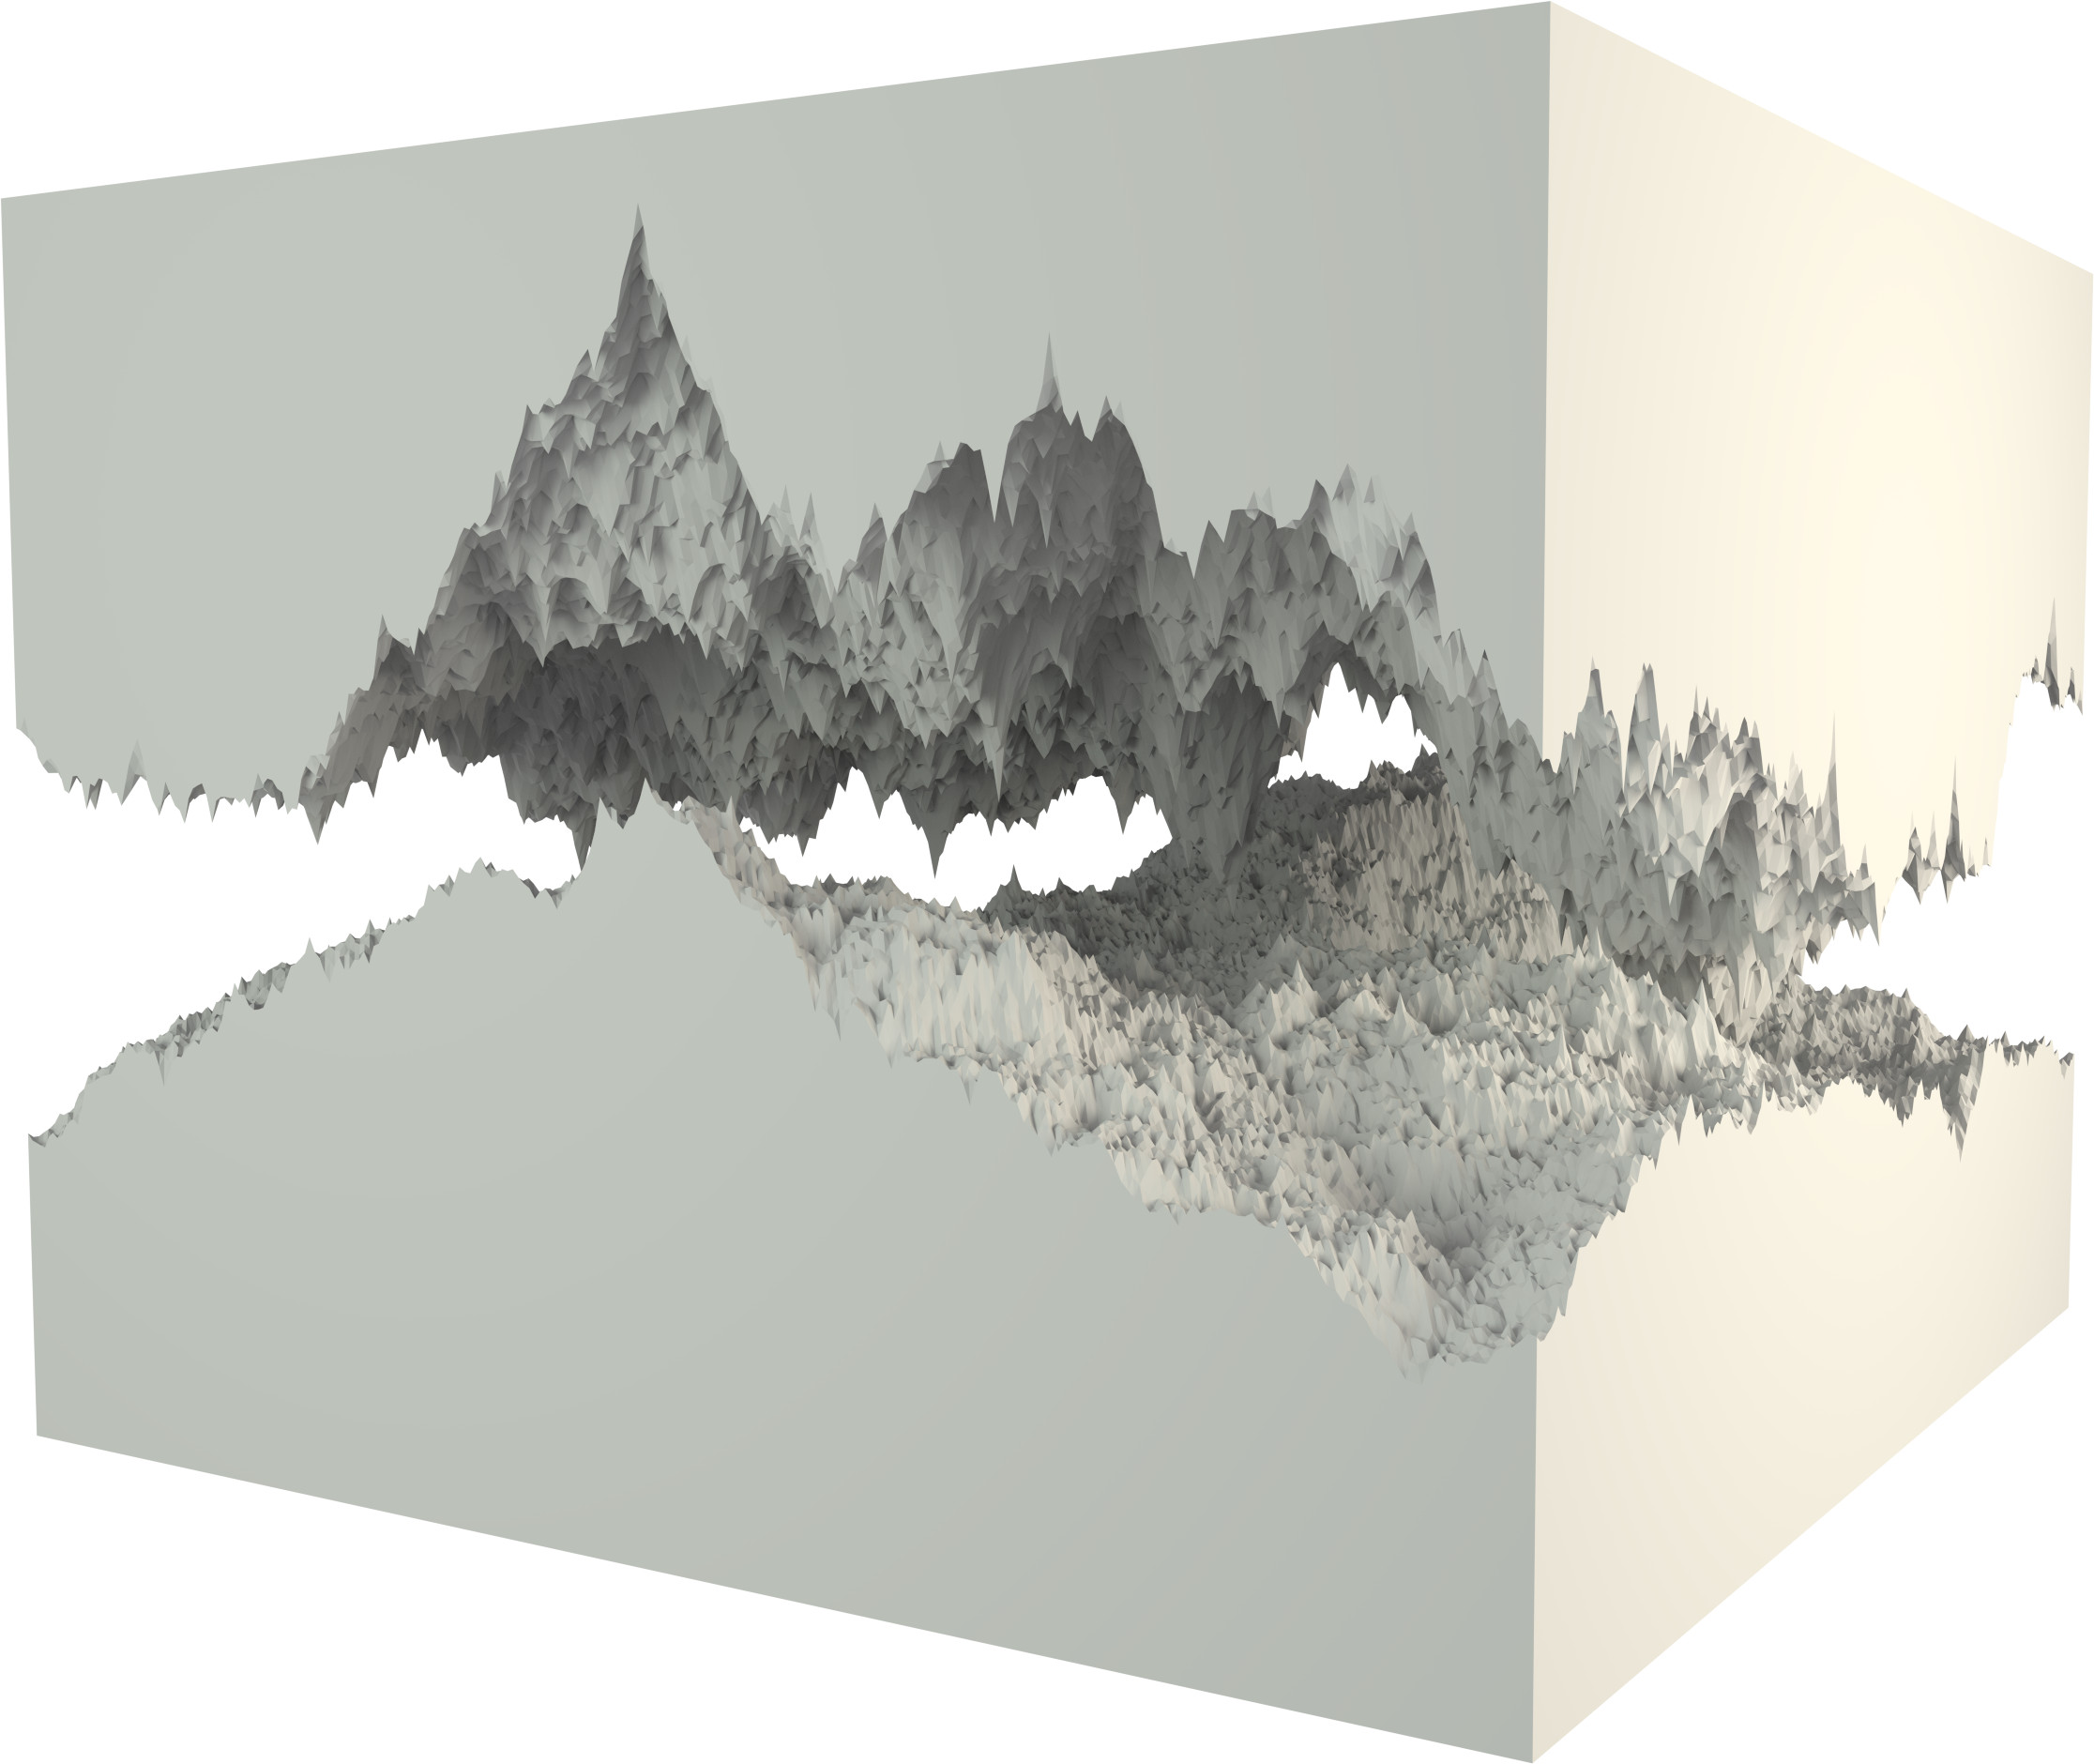
\includegraphics[width=\textwidth]{images/fracture/large_fracture05}
    \caption{Caption}
\end{figure}

We want to study the behaviour of water trapped in nanoscale (pores and) fractures in silica, so need want a way to generate and characterize such a structure. (Several methods of characterizing a fracture could be imagined (\hl{SOURCES, examples}), and we will use several of them.)        

\hl{terrain == heightmap??, finn bra ord her}

\section{Characterization}

\todo{change wording? copied from Fractals...}
An \emph{affine transformation} transforms a point $\bvec x = (x_1, \dots, x_n)$ into new points $\bvec x' = (r_1x_1, \dots, r_n, x_n)$, where the scaling rations $r_1, \dots, r_n$ are \emph{not} all equal.

A bounded set $\mathcal{S}$ is \emph{self-affine} if $\mathcal{S}$ is the union of $N$ non-overlapping subsets $\mathcal{S}_1, \dots, \mathcal{S}_N$, each of which is congruent to the set $\bvec r(\mathcal{S})$ obtained from $\mathcal S$ by the affine transform defined by $\bvec r$. Here \emph{congruent} means that the set of points $\mathcal{S}$ is identical to the set of points $\bvec r(\mathcal{S})$ after possible translations and/or rotations of the set\cite{feder1988fractals}.

A set $\mathcal{S}$ is \emph{statistically self-affine} if $\mathcal{S}$ is the union of $N$ non-overlapping subsets each of which is scaled down by $\bvec r$ from the original, and is identical in all statistical respects to $\bvec r(\mathcal{S})$.

\subsection{Hurst exponent}
\orangebox{
\begin{itemize}
    \item define fractal dimension
\end{itemize}
}

To characterize a fractal one can use the Hurst exponent, usually called $H$\footnote{\todo[inline]{The name used by Hurst in his work where he first describes the exponent was actually $K$\cite{hurst1965longterm}\cite{hurst1951longterm}}}, which comes from a statistical method developed by Hurst\cite{hurst1965longterm}\cite{hurst1951longterm}. The Hurst exponent is related to the fractal dimension $D$ by
\begin{align*}
    D = d-H,
\end{align*}
where $d$ is the spatial dimension of the fractal's domain\cite{feder1988fractals}.

The statistical method developed by Hurst is called \emph{rescaled range analysis} and was designed for use on 1-dimensional time series $f(t)$. The method has been generalized to higher dimensions\cite{fan2013rescaled}, but the original 1D form is shown here.

\subsubsection{Rescaled range analysis}
First the time series is divided into \todo{overlapping/non-overlapping?} intervals of length $\tau$. The average over each interval of length $\tau$ is
\begin{align*}
    \langle f \rangle_\tau = \frac{1}{\tau} \sum_{t=1}^\tau f(t).
\end{align*}
We let $F$ be the accumulated deviation from the mean
\begin{align*}
    F(t, \tau) = \sum_{t' = 1}^t \big( f(t') - \langle f \rangle_\tau \big).
\end{align*}
The difference between the maximum and minimum of the accumulated deviation from the mean is the \emph{range} R
\begin{align*}
    R(\tau) = \max_{1 \leq t \leq \tau} \big(F(t,\tau)\big) - \min_{1 \leq t \leq \tau} \big(F(t, \tau)\big).
\end{align*}
The standard deviation $S$ of the time series is estimated using
\begin{align*}
    S^2 = \frac{1}{\tau} \sum_{t=1}^\tau \big( f(t) - \langle f \rangle_\tau \big)^2.
\end{align*}
Hurst found that the observed \emph{rescaled range}, $R/S$, for many time series is described by the \hl{empirical} relation\cite{feder1988fractals}
\begin{align*}
    \frac{R}{S} = \left(\frac{\tau}{2}\right)^H \sim \tau^H.
\end{align*}
We now see that we can estimate the Hurst exponent by a linear fit of the form
\begin{align*}
    \log \left(\frac{R}{S}\right) \sim H\log\tau,
\end{align*}
where we find $H$ as the slope of the linear fit.

\todo[inline]{Something about that it's hard to measure, and why.}

\subsubsection{Detrending moving average}
To estimate the Hurst exponent of a surface we use a method called detrending moving average (DMA) first described by E. Alessio, A. Carbone et al.\cite{alessio2002dma}, and later generalized to higher dimensions by A. Carbone \cite{carbone2007algorithm}. We use this method because ??? \todo[inline]{good results, easy to implement? }

We define a \hl(self-affine) surface as $f(i,j)$, where $f$ is the height in the point $(i,j)$, defined in a discrete 2-dimensional domain with size $N\times N$, and with $i,j = 1,\dots,N$. We divide the surface into square \hl{subsurfaces} of size $n \times n$, and find the average $\tilde f_n$ of each subsurface by\footnote{\cref{eq:carbone_average} is how the average $\tilde f_n$ is stated in the article\cite{carbone2007algorithm}, but we rewrite it to \cref{eq:carbone_average_rewritten} so it's easier to understand. The two forms are equivalent.}
\begin{align}
    \tilde f_n(i,j) 
    &= \frac{1}{n^2}\sum_{k=-m}^{n-1-m} ~ \sum_{l=-m}^{n-1-m} f(i-k, j-l) \label{eq:carbone_average}\\
%     &= \frac{1}{n^2}\sum_{k=i-m}^{i-n+1+m}\sum_{l=j-m}^{j-n+1+m} f(i-k, j-l) \\
    &= \frac{1}{n^2} \sum_{k=(i+m)-n+1}^{i+m} ~ \sum_{l=(i+m)-n+1}^{i+m} f(k, l), \label{eq:carbone_average_rewritten}
\end{align}
where
\begin{align*}
    &m = \left \lfloor n\theta \right \rfloor &\text{for }0 \leq \theta < 1,
\end{align*}
which means that $0 \leq m \leq (n-1)$. $\theta$ is a parameter that controls the position of the square relative to the point $(i,j)$ in $\tilde f_n(i,j)$. There are three \hl{extreme} cases for $\theta$, which are listed below, and are illustrated in \cref{fig:DMA_theta}.
% \begin{itemize}
%     \item For $\theta = 0$ we have $m=0$ and we average over a square with the point $(i,j)$ in the square's upper right corner (($i-n+1) \leq k,l \leq i$). See \cref{fig:DMA_theta_a}.
%     \item For $\theta = 1/2$ we average over a square centered on the point $(i,j)$. See \cref{fig:DMA_theta_b}.
%     \item For $\theta = (n-1)/n$ we have the maximum value for $m$, $m=n-1$, and average over a square with the point $(i,j)$ in the square's lower left corner \todo{THESE LIMITS ARE WRONG??}($i \leq k,l \leq (i+n-1)$). See \cref{fig:DMA_theta_c}.
% \end{itemize}
\begin{description}
    \item[$\bm{\theta = 0}$:] \hfill\\ 
        We have $m=0$ and we average over a square with the point $(i,j)$ in the square's upper right corner (($i-n+1) \leq k,l \leq i$). See \cref{fig:DMA_theta_a}.
    \item[$\bm{\theta = 1/2}$:] \hfill\\ 
        We average over a square centered on the point $(i,j)$. See \cref{fig:DMA_theta_b}.
    \item[$\bm{\theta = (n-1)/n}$:] \hfill\\ 
        {\sloppy 
        We have the maximum value for $m$, $m=n-1$, and average over a square with the point $(i,j)$ in the square's lower left corner \todo{\st{THESE LIMITS ARE WRONG??} fixed}\\(${i \leq k,l \leq (i+n-1)}$). See \cref{fig:DMA_theta_c}.
        }
\end{description}

\begin{figure}
    \centering
    \begin{subfigure}[b]{0.25\textwidth}
        \includesvg[width=\textwidth, svgpath=./images/Hurst/]{2DDMA_theta04_a}
%         \caption{Illustration of how to divide a convex hexahedron into five tetraheda.}
        \caption{$\theta = 0$}
        \label{fig:DMA_theta_a}
    \end{subfigure}
    \hspace{0.1\textwidth}
    \begin{subfigure}[b]{0.25\textwidth}
        \includesvg[width=\textwidth, svgpath=./images/Hurst/]{2DDMA_theta04_b}
%         \caption{A random fracture made from two periodic heightmaps.}
        \caption{$\theta = 1/2$}
        \label{fig:DMA_theta_b}
    \end{subfigure}
    \hspace{0.1\textwidth}
    \begin{subfigure}[b]{0.25\textwidth}
        \includesvg[width=\textwidth, svgpath=./images/Hurst/]{2DDMA_theta04_c}
%         \caption{A random fracture made from two periodic heightmaps.}
%         \caption{$\theta \rightarrow 1$ \\ ($\theta = (n-1)/n$)}
%         \caption{$\theta \rightarrow 1$}
        \caption{$\theta = (n-1)/n$}
        \label{fig:DMA_theta_c}
    \end{subfigure}
        \caption{
        Illustration of what the parameter $\theta$ controls in the detrending moving average method in 2 dimensions. The circles are points where the surface is defined, the red star is the point $(i,j)$, and the black square encompasses the points averaged over to calculate $\tilde f_n(i,j)$ in \cref{eq:carbone_average_rewritten}. The illustration uses $n = 3$.
        \label{fig:DMA_theta}
    }
\end{figure}

We then define the generalized variance $\sigma_\text{DMA}^2$
\begin{align*}
    \sigma_\text{DMA}^2 
    = \frac{1}{(N-n)^2}\sum_{i=n-m}^{N-m} ~ \sum_{j=n-m}^{N-m} 
    \big(
        f(i,j) - \tilde f_n(i,j)
    \big)^2,
\end{align*}
where we see that $f(i,j) - f_n(i,j)$ is the difference between the point $(i,j)$ and the average of a square of points (including the point itself) of size $n \times n$, as explained above (see \cref{fig:DMA_theta}).
% (the position of the square is controlled by the parameter $\theta$, as explained above, and illustrated \cref{fig:DMA_theta}). 
The summation limits $(n-m) \leq i,j \leq N-m$ are set so that the averages $f_n(i,j)$ don't exceed the domain with size $N \times N$.

The generalized variance goes as
\begin{align*}
    \sigma_\text{DMA}^2 \sim \left(2n^2\right)^H,
\end{align*}
which we can use to find the Hurst exponent $H$, by calculating $\sigma_\text{DMA}^2$ for different sizes of the squares, $n$. We estimate $H$ by a linear fit of $\log \sigma_\text{DMA}^2$ against $\log 2n^2$, where $H$ is the slope.

In the paper that generalizes DMA to higher dimensions\cite{carbone2007algorithm} they use different parameters for each spatial dimension $d$, $\bvec\theta = \theta_1, \dots, \theta_d$ and $\bvec{n} = n_1, \dots, n_d$, but for simplicity and to avoid \hl{strange} results, we use $\theta_1 = \theta_2 = \theta$ and $n_1 = n_2 = n$.

% With $\theta = 0$ we have $m = 0$ and average over all points $(\leq k \leq i,l \leq j)$. 

% With $\theta = n/(n-1)$ we have $m = n-1$, and average over all points $(k \geq i,l \geq j)$.

% We define the generalized variance $\sigma_\text{DMA}^2$ as the variance 
% \begin{align*}
%     \sigma_\text{DMA}^2 
%     = \frac{1}{(N-n)^2}\sum_{i=n-m}^{N-m}\sum_{j=n-m}^{N-m} 
%     \big(
%         f(i,j) - \tilde f_n(i,j)
%     \big)^2,
% \end{align*}
% where\footnote{We rewrite \cref{eq:carbone_average} for easier understanding}
% \begin{align}
%     \tilde f_n(i,j) 
%     &= \frac{1}{n^2}\sum_{k=-m}^{n-1-m}\sum_{l=-m}^{n-1-m} f(i-k, j-l) \label{eq:carbone_average}\\
% %     &= \frac{1}{n^2}\sum_{k=i-m}^{i-n+1+m}\sum_{l=j-m}^{j-n+1+m} f(i-k, j-l) \\
%     &= \frac{1}{n^2} \sum_{k=(i+m)-n+1}^{i+m} ~ \sum_{l=(i+m)-n+1}^{i+m} f(k, l).\nonumber %\label{eq:carbone_average_rewritten}
% \end{align}
% \begin{align*}
%     m = \left \lfloor n\theta \right \rfloor
% \end{align*}
% $\theta = 1$ or $\theta = 0$ (directed implementation, for fractals with preferential growth direction) \\
% $\theta = 0.5$ (isotropic implementation, ``uniformity in all orientations'') \\



% \begin{figure}
%     \centering
%     \includesvg[width=0.99\textwidth, svgpath=./images/Hurst/]{2DDMA_theta04}
%     \caption{
%         Illustration of what the parameter $\theta$ controls in the detrending moving average method in 2 dimensions. The circles are points where a surface is defined, the red star marks the point $(i,j)$, and the black square marks the points averaged over to calculate $\tilde f_n(i,j)$ in \cref{eq:carbone_average_rewritten}.
%         \label{fig:DMA_theta}
%     }
% \end{figure}



% \subsubsection{Detrended fluctuation analysis in higher dimensions}
% original DFA\cite{peng1994mosaic}
% HDDMA\cite{gu2006detrended}
% 
% To estimate the Hurst exponent of a fracture we use a generalized version of a method called \emph{detrended fluctuation analysis}\cite{peng1994mosaic}, which was generalized to higher dimensions by Gu and Zhou\cite{gu2006detrended}.
% 
% The two-dimensional DFA:
% 
% We have a self-affine surface stored in the matrix $f(i,j)$, where $f$ \hl{is} the height of the surface in the point $(i,j)$, with $i,j = 1,\dots,N$, and $N^2$ is the number of points where the surface is defined. The surface is divided into $n\times n$ disjoint (non-overlapping) \hl{and neighboring} surfaces \todo{sub-surface?} of the same size $s\times s$, where $n = N/s$. Each of these surfaces is denoted by $f_{u,v}$ such that $f_{u,v}(i,j) = f(i+k, j+l)$ for $i,j = 1, \dots, s$, where $k = (u-1)s$ and $l = (v-1)s$.
% 
% For a surface $f_{u,v}$ the cumulative sum $F_{u,v}(i,j)$ is calculated as follows
% \begin{align*}
%     F_{u,v}(i,j) = \sum_{m=1}^i\sum_{n=1}^j f_{u,v}(m,n),
% \end{align*}
% where $i,j = 1,\dots,s$. Note that F_{u,v}(i,j) itself is a surface.
% 
% The trend of the constructed surface $F_{u,v}$ can be determined by fitting it with a polynomial $\tilde F$



\todo[inline]{implemented in Matlab/Octave}

\subsection{Surface area}
\subsection{Distance to nearest atom}
\begin{itemize}
    \item Fractals
    \item Fractional Brownian Motion
    \item The Hurst Exponent
\end{itemize}

\section{Generating fractures}
\hl{Stuff to define?}
\begin{itemize}
    \item fBm surfaces
    \item Hurst exponent
    \item Gaussian random variable ?
    \item non-stationary
    \item self-similar
    \item isotropic
    \item lacunarity
\end{itemize}

\subsection{Generating surfaces}
% When generating random surfaces we want to be able to control the properties like the Hurst exponent (\hl{etc.?}) of the surface.

To generate our random surfaces we use an iterative midpoint displacement method usually called successive random additions \hl{(SRA)}. The method is based on a method proposed by Fourner in 1982\cite{fournier1982computer}, but with some modifications suggested by Voss\cite{voss1985random, voss1988fractals}. The method has further been discussed by Saupe\cite{saupe1988algorithms}, amongst others. We choose this method mainly because it's possible to generate periodic surfaces with it, because it generates very good approximations to fBm surfaces\cite{zhou2005comparison}, and because the Hurst exponent of the generated surfaces is easy to control. The method is also easy to understand, easy to implement, and generates surfaces with high resolution very fast. The method is widely used in scientific applications\hl{cite??} because of these properties, and is also used for generating surfaces in computer graphics, since the surfaces look very realistic \hl{with only some minor artefacts?? (high, narrow peaks)}.

\subsubsection{Midpoint displacement method in 1 dimension}
The method we use to generate random surfaces is very similar to the standard midpoint displacement method, which in 1 dimension goes as follows. See \cref{fig:midpoint01} for a visual presentation.
\begin{enumerate}
    \item Give the values at the endpoints of the interval, $y_0$ and $y_n$, random values from a Gaussian random variable with mean $\mu = 0$ and variance $\sigma_0^2$. This initial standard deviation $\sigma_0$ can be chosen freely.
    \item Generate the value in the center of the interval, $y_{n/2}$, by averaging over the two endpoints and adding a Gaussian random number with mean $\mu = 0$ and a \emph{reduced} variance
    \begin{align}
         \sigma_1^2 = \left(1/2\right)^{2H}\sigma_0^2, \label{eq:midpoint_sigma_first}
    \end{align}
    where $H$ is the wanted Hurst exponent.
    \item Continue generating the values in the center of each sub-interval until you reach the desired number of points, while reducing the variance of the random number by a factor $\frac{1}{2}$ each iteration\todo{Why 1/2? (needed to create good fBm, see \cite{voss1985random})}. For iteration $i$ we have
    \begin{align}
        \sigma_i^2 = \left(1/2\right)^{i2H}\sigma_0^2. \label{eq:midpoint_sigma_general}
    \end{align}
\end{enumerate}

\begin{figure}
    \centering
    \includesvg[width=0.5\textwidth, svgpath=./images/diamond_square/]{random_midpoint_displacement_regular02}
    \caption{
        \hl{Illustration of the midpoint displacement method in 1 dimension.}
        \label{fig:midpoint01}
    }
\end{figure}

This method generates a \hl{1-dimensional line}, with a Hurst exponent \hl{close} to the input $H$\todo{how close?}. But since we only add random numbers to the new values, the result is non-stationary for $H \neq 0.5$\cite{voss1985random}\hl{, and it is neither self-similar or isotropic, as noted by Mandelbrot}\cite{mandelbrot1982comment}. To mitigate this we implement the addition suggested by Voss\cite{voss1985random}, which consists of adding a random number to \emph{all} points in each iteration, both the new and old. Voss called this modified method \emph{successive random additions}.

\subsubsection{Successive random additions \hl{(on an infinite grid)} in 2 dimensions}
As mentioned before, the method called \emph{successive random additions} is a modification of the regular midpoint displacement method first described by Richard F. Voss\cite{voss1985random}, where we add random numbers to \emph{all} points in each iteration, compared to just the \emph{new} points in the regular midpoint displacement method. This modification means that we can replace the factor $(1/2)$ in \cref{eq:midpoint_sigma_first,eq:midpoint_sigma_general} with a general factor $r$\todo{why? (something about distance between points)}, and we get
\begin{align*}
    \sigma_i^2 = r^{2H}\sigma^2_{i-1}.
\end{align*}
\hl{$r$ controls the lacunarity/roughness, $H$ independent of $r$}

Voss has geneneralized the the method of successive random additions to higher dimensions\cite{voss1985random}, and this generalized form is the algorithm we use when generating fractures. We generate surfaces in the form of heightmaps, meaning a 2-dimensional grid of points ({$x,y$}), with a value for the height in each point \hl{($z(x,y) = z_{x,y}$)} which is generated by the algorithm.

The central part of the algorithm consists of two steps often called the \emph{diamond-step} and the \emph{square-step}. We start with a simple case of an infinite grid of evenly spaced points, all with known $z$-values. The two steps are as follows:
\begin{description}
    \item[The \emph{square-step}:] The grid can be divided into small squares consisting of four points in each square, as in the leftmost square in \cref{fig:simple_square_step}. We generate the $z$-value in the center of each of these squares by averaging the $z$-values of the four corners of each square, as indicated by the red dots and arrows in \cref{fig:simple_square_step}. Then add a random Gaussian number with mean $\mu = 0$ and variance $\sigma_i^2 = \sigma_{i-1}^2r^{2H}$ to all new and old points, where $\sigma_{i-1}^2$ is the variance used in the last step of the algorithm.
    \label{enum:test}
    
    \item[The \emph{diamond-step}:] After the square-step the grid can be divided into smaller squares that are tilded by 45 degrees, as in the leftmost square in figure \cref{fig:simple_diamond_step}. We generate the $z$-values in the center of each square by averaging the $z$-values of the four corners of each square, as indicated by the red dots and arrows in \cref{fig:simple_diamond_step}. We then add a random Gaussian number with mean $\mu = 0$ and variance $\sigma_{i+1}^2 = \sigma_i^2r^{2H}$, to all new and old points. 
\end{description}
See \cref{fig:diamond_square_applied} for an illustration of the algorithm applied once on a larger grid. 

\begin{figure}
\centering

\setlength{\myfigwidth}{0.5\textwidth}
\setlength{\mycaptionwidth}{0.3\textwidth}

\begin{minipage}[c]{\myfigwidth}
    \includesvg[width=\textwidth, svgpath = images/diamond_square/]{simple_square_step_solarized08}
\end{minipage}
\begin{minipage}[c]{\mycaptionwidth}
    \subcaption{Square-step}
    \label{fig:simple_square_step}
\end{minipage}

\begin{minipage}[c]{\myfigwidth}
    \includesvg[width=\textwidth, svgpath = images/diamond_square/]{simple_diamond_step_solarized05}
\end{minipage}
\begin{minipage}[c]{\mycaptionwidth}
    \subcaption{Diamond-step}
    \label{fig:simple_diamond_step}
\end{minipage}

\caption{Illustration of the two steps used in the diamond square algorithm for generating random surfaces. The grey points are old points, the black points are new points, and the red points are the points used in the calcuation of the averages when generating the new points.}
\label{fig:diamond_square_steps}
\end{figure}

We see that by first applying the square-step and then applying the diamond-step, we add one point in between each point in each direction, almost doubling the resolution of the grid. In general we go from $n$ to $n + (n-1)$ points in each direction. By applying the algorithm several times we get \todo{replace $n$ with $N$ and $i$ with $n$?}
\begin{align}
    n_1 &= n_0 + (n_0-1) = 2n - 1 \nonumber\\
    n_2 &= 2n_1 - 1 = 4n_0 - 3 \nonumber\\
    n_3 &= 2n_2 - 1 = 9n_0 - 7 \nonumber\\
    &\vdotswithin{=} \nonumber\\
%     &\shortvdotswithin{=}
    n_i &= 2^i(n_0-1) + 1, \label{eq:diamond_step_resolution}
\end{align}
where $i$ is the number of times we have applied the algorithm. This means that using the diamond-square algorithm we can go from any resolution $n_0$ to all resolutions satisfying $n_i = 2^i(n_0 - 1) + 1$.

\begin{figure}
    \centering
    \includesvg[width=0.7\textwidth, svgpath = images/diamond_square/]{increase_resolution_solarized_starssquares03}
    \caption{
        The diamon-square algorithm applied once on a grid of $3\times 3$ points, increasing the number of points from 9 to 25. The orange square points are generated by the square-step (see \cref{fig:simple_square_step}), and the blue star-shaped points by the diamond-step (see \cref{fig:simple_diamond_step}).
    }
    \label{fig:diamond_square_applied}
\end{figure}

\subsubsection{Successive random additions on a finite grid \hl{in 2 dimensions}}
Since we are using computers to generate our surfaces, which have limited memory, we can't use infinite grids. This means we get some special cases that needs to be taken care of when generating points near the edges of the grid.\todo{transition to below}

For the square step we generate one new point in the center each square formed by the grid from the previous iteration, and in general we generate the $z$-values in the points
\begin{align}
    &\left(x_{i+1/2}, y_{j+1/2}\right) &0\leq i,j < n, \label{eq:square_step_limits}
\end{align}
where $(x_i,x_j)$ are the points in the grid after the last iteration. In general the averages we calculate for the new points can be written as\todo{make this equation nicer}
% \begin{align}
%     (x_{i+1/2}, y_{j+1/2}) 
%     &= \frac{1}{4}\big(
%         (x_i, y_j) + (x_{i+1}, y_j)\nonumber\\
%         &+ (x_i, y_{j+1}) + (x_{i+1}, y_{j+1})
%     \big)
%     &0\leq i,j < n.
%     \label{eq:square_step}
% \end{align}
\begin{align}
    (x_{i+1/2}, y_{j+1/2}) 
    = \frac{1}{4}\big[
        (x_i, y_j) + (x_{i+1}, y_j)
        &+ (x_i, y_{j+1}) + (x_{i+1}, y_{j+1})
    \big],
    \label{eq:square_step}
\end{align}
using the limits in \cref{eq:square_step_limits}. We see that the square-step only uses points inside the grid, which means that we don't have to modify it when going to a finite grid.

For the diamond-step we generate the values in the points

\begin{align}
    &(x_{i+1/2}, y_j) &\text{for } 0\leq i<n \text{ and } 0\leq j \leq n& \label{eq:diamond_step_limits01}\\
    &(x_i, y_{j+1/2}) &\text{for } 0\leq i\leq n \text{ and } 0\leq j < n&. \label{eq:diamond_step_limits02}
\end{align}
In general the averages we calculate for the new points can be written as\todo{make these equations nicer}
% \begin{align}
%     (x_{i+1/2}, y_j) 
%     &= 
%     \frac{1}{4}\big(
%         (x_i, y_j) + (x_{i+1}, y_j) + (x_{i+1/2}, y_{j-1/2}) + (x_{i+1/2}, y_{j+1/2})
%     \big) \label{eq:diamond_step01}\\
%     (x_i, y_{j+1/2}) 
%     &= 
%     \frac{1}{4}\big(
%         (x_i, y_j) + (x_i, y_{j+1}) + (x_{i-1/2}, y_{j+1/2}) + (x_{i+1/2}, y_{j+1/2})
%     \big). \label{eq:diamond_step02}
% \end{align}
\begin{align}
    (x_{i+1/2}, y_j) 
    &= 
    \frac{1}{4}\big[
        (x_i, y_j) + (x_{i+1}, y_j) \nonumber\\
        &+ (x_{i+1/2}, y_{j-1/2}) + (x_{i+1/2}, y_{j+1/2})
    \big]
    \label{eq:diamond_step01}\\
    (x_i, y_{j+1/2}) 
    &= 
    \frac{1}{4}\big[
        (x_i, y_j) + (x_i, y_{j+1}) \nonumber\\
        &+ (x_{i-1/2}, y_{j+1/2}) + (x_{i+1/2}, y_{j+1/2})
    \big],
    \label{eq:diamond_step02}
\end{align}
using the limits in \cref{eq:diamond_step_limits01,eq:diamond_step_limits02}. We now see that when generating points near the edges using the diamond-step, specifically when generating the points $(x_{i+1/2}, y_j)$ for $j \in \{0, n\}$ and $(x_i, y_{j+1/2})$ for $i = \{0, n\}$, we need to average over points that lie outside the grid. There are two possible solutions, depending on the surface we are generating. If generating a periodic surface, the solution is to wrap around the edges using periodic boundary conditions, and find the point we need on the opposite side of the grid. For example (using $i = j = 0$)
\begin{align*}
    (x_{1/2}, y_{-1/2}) = (x_{1/2}, y_{n-1/2}).
\end{align*}
If generating a non-periodic grid we simply ignore the points that lie outside the grid when calculating the averages, and just use the \hl{three/3} other points.

\subsubsection{Implementing successive random additions \hl{on a finite grid in 2 dimensions}}
In our implementation we generate a surface on a finite grid of size $N\times N$, starting with only the $z$-values in the four corners defined, giving a resolution $n_0 = 2$. As shown in \cref{eq:diamond_step_resolution} the algorithm can go from any resolution $n_0$ to any resolution \hl{of the form} $n_p = 2^p(n_0-1) + 1$ by applying the algorithm $p$ times, which means that our implementation can generate surfaces with resolutions
\begin{align*}
    N &= 2^p(2-1) + 1 = 2^p + 1,
\end{align*}
where $p$ is any positive integer.

We implement generation of both periodic and non-periodic surfaces using using \crefrange{eq:square_step_limits}{eq:diamond_step02}, while skipping points outside the grid for non-periodic surfaces, and wrapping around the edges using periodic boundary conditions when generating periodic surfaces.

To ensure that the periodic surfaces actually turn out periodic we start with all four corners having the same value. We also let the right and bottom edge be equivalent to the left and top edge, respectively, which effectively means that all four corners should always have the same $z$-value. To ensure that the opposite edges stay equal to each other we never generate any points on the right and bottom edge, but just copy the $z$-values from the opposite \hl{corresponding} edge after the diamond-step.

This leaves us with the following algorithm for generating a surface which approximates a 2-dimensional fractional Brownian motion with Hurst exponent $H$
\begin{enumerate}
    % \itemsep1pt \parskip0pt \parsep0pt
    \renewcommand{\labelitemii}{$\bullet$}
    
    \item Allocate a grid of size $N\times N$, where $N = 2^p + 1$, and $p$ is any positive integer. This grid will store the $z$-values, or the height of the surface, in each grid point $(x,y)$.

    \item Initialize the values in the corners of the grid by drawing random numbers from a Gaussian distribution with mean $\mu = 0$ and variance $\sigma_0$. The initial variance can be chosen freely. \hl{The initial resolution is now $n_0\times n_0$, with $n = 2$}.
    \begin{itemize}
        \item If generating a periodic surface, give all four corners the same $z$-value.
    \end{itemize}
    
    \item Apply the square-step using \cref{eq:square_step_limits,eq:square_step}. Add a random Gaussian number with mean $\mu = 0$ and variance $\sigma_i = \sigma_{i-1}^2r^{2H}$ to all new and old points.
    \label{enum:square_step}

    \item Apply the diamond-step using \crefrange{eq:diamond_step01}{eq:diamond_step02}. Add a random Gaussian number with mean $\mu = 0$ and variance $\sigma_{i+1} = \sigma_i^2r^{2H}$ to all new and old points.
    \label{enum:diamond_step}
    
    \begin{itemize}
        \item If generating a periodic surface, skip generating points on the right and bottom edge using the diamond-step, and instead copy the $z$-values from the opposite edges.
    \end{itemize}
    
    \item Repeat step \ref{enum:square_step} and \ref{enum:diamond_step} $p$ times until you reach the desired resolution of $N\times N$, where $N = 2^p + 1$. For step $i$ the variance of the random Gaussian numbers is
    \begin{align*}
        \sigma_i^2 = \sigma_0^2(r^i)^{2H}.
    \end{align*}
    
%     Continue generating new points and increasing the resolution of the surface until you reach the desired number of \hl{points/resolution}. We see in \cref{fig:square_step} that the square step doesn't need any changes, since we don't generate any points at the edges of the grid, and we never have any neighbors that are beyond the edges of the grid. For the diamond step we need to make sure we wrap around the edges to find neighbors when calculating points that are close to the edges of the grid, and that we update the left and bottom edges as needed. 
    
%     \item Generate the $z$-value in the center of each square \hl{of defined points} of size $n_i = 2^i + 1$ using \cref{eq:square_step_limits,eq:square_step}.
    
%     \item Generate the $z$-value in the center of each square \hl{of defined points} of size $n_i = 2^i + 1$ using \crefrange{eq:diamond_step01}{eq:diamond_step02}.
    
%     \item Generate the $z$-value in the center of each square of already defined points by using the square-step, as in \cref{fig:square_step}. Add a random Gaussian value with mean $\mu = 0$ and variance $\sigma_0^2$ to all new and old points. The initial standard deviation $\sigma_0$ can be chosen freely. 
    
%     \item Generate the $z$-value in the center of the grid using the square step by averaging over the four corners, as shown in \cref{fig:initial_square_step}. Add a random Gaussian number with mean $\mu = 0$ and variance $\sigma_1^2 = \sigma_0^2r^{2H}$\todo{define r} to the new point, and to the four corners (add the same number to all four corners to keep the system periodic).
    
%     \item Generate the values in the middle of the top and left edge of the grid using the diamond step, as shown in \cref{fig:diamond_step}. Add a random Gaussian number with mean $\mu = 0$ and variance $\sigma_2^2 = \sigma_1^2r^{2H}$ to all new and old points. Set the point in the middle of the right and bottom edges equal to 
    
%     When calculating the averages in the diamond-step  Since the surface is periodic, we can wrap around the edges to reach the points beyond the edges of our grid (the points outside the grid in \cref{fig:diamond_step}). Set values in the middle of the right and bottom edge equal to the corresponding values in the middle of the left and top edge, to keep the surface periodic\footnote{\hl{We could have done this in a slightly different way, by making the grid one unit smaller, and starting with only one point in one of the corners, but by doing it the way we have we can keep the square step the same as before.}}.
    
%     \item We now need to generate the $z$-values in the middle of the four edges of the grid, using the diamond step. But since we have a finite and periodic grid, we have to wrap around the edges when taking the average over the four neighbours. We also see that the top and bottom edge, and the left and right edge should be equal after generating the new points\footnote{\hl{We could have done this in a slightly different way, by making the grid one unit smaller, and starting with only one point in one of the corners, but doing it the way we have we can keep the square step the same as before.}}, to keep the grid periodic. This can for example be done by generating the point in the middle of the left edge and the point in the middle of the top edge by using the diamond step and wrapping around the edges, and then setting the corresponding points on the right and bottom edge equal to the generated points.
    
%     This can for example be done by only generating the points on the top and left edge, and then setting the points on the right edge equal to the left edge, and the points on the .

%     \item Continue generating new points and increasing the resolution of the \hl{surface/grid} until you reach the desired number of \hl{points/resolution}. We see in \cref{fig:square_step} that the square step doesn't need any changes, since we don't generate any points at the edges of the grid, and we never have any neighbors that are beyond the edges of the grid. For the diamond step we need to make sure we wrap around the edges to find neighbors when calculating points that are close to the edges of the grid, and that we update the left and bottom edges as needed. 
%     
%     For step $i$ the variance of the random Gaussian number is
%     \begin{align*}
%         \sigma_i^2 = \sigma_0^2(r^i)^{2H}.
%     \end{align*}
\end{enumerate}

See \cref{fig:diamond_square_surface} for a surface generated by the algorithm.

\begin{figure}
    \centering
    \includesvg[width=0.7\textwidth, svgpath=./images/diamond_square/surface_example/]{surface_labels}
    \caption{
        Caption.
        \label{fig:diamond_square_surface}
    }
\end{figure}

On a computer we would like to allocate a matrix for storing each point in the final surface before using the algorithm, which means we have to know the size beforehand.

In our implementation of the algorithm we start from a grid with the $z$-value in each corner defined (a resolution of $2\times 2$), which means our final resolution is $n_i = 2^i + 1$ after $i$ iterations, and that we should allocate a matrix of size $(2^i + 1) \times (2^i + 1)$ in the initialization of the program.

\orangebox{
{\bf Notes:}
\begin{itemize}
    \item Implementation (in Matlab/C++)?
    \item periodic and non-periodic
    \item Mention that DS can be used to increase resolution of any surface
    \item Can increase resolution of generated surface, if we know the seed
\end{itemize}

{\bf Stuff to define:}
\begin{itemize}
    \item Periodic/non-periodic
    \item Lacunarity
\end{itemize}
}

% \begin{figure}
%     \centering
%     \def\svgwidth{\textwidth}
%     \input{images/diamondSquare02.eps_tex}
% \end{figure}

% \begin{figure}
%     \centering
%     \def\svgwidth{\textwidth}
%     \input{images/diamondSquare03.pdf_tex}
% \end{figure}

% \subsection{Successive Random Addition}
% To generate a random heightmap with a known Hurst exponent we used the successive random addition (SRA) algorithm introduced by Voss\cite{voss1985random}. It is a variation of a simpler algorithm called random midpoint displacement (RMD), a subdivision method described by, amongst others, Fournier, Fussell, and Carpenter\cite{fournier1982computer, carpenter1980computer}. To illustrate how the algorithms work, we will start with a simple 1-dimensional example of RMD.
% 
% We start with two points $Y(0)$ and $Y(1)$ at the edges of our interval. We find a point $Y(\frac{1}{2})$ in the center of the interval by interpolating the two initial points, and adding a Gaussian random number with zero mean and variance $\sigma^2$
% 
% \subsection{Midpoint Displacement Method}
% The most basic method we used is a very basic but widely used method, which has many variations and names. The most common names are ``the diamond-square algorithm''\hl{cite}, ``the midpoint displacement method''\hl{cite}, ``plasma fractal'' and ``cloud fractal''.
% 

\subsection{Generating fractures from surfaces}
To generate a realistic fracture we use the method of successive random additions, as described previously, to generate random heightmaps with a known Hurst exponent. If we generate two of these surfaces we can make a fracture by putting one surface above the other, and letting either the space between or outside the heightmaps be the void. Since we are using periodic systems the two different approaches are equivalent, but we chose to let the space between the heightmaps be the void, for easier visualization.

In practice we make a fracture using the following procedure
\begin{itemize}
    \item Generate two heightmaps.
    \item Rescale the $x$- and $y$-positions of all points in the heightmaps, so they span the size of the atomic system.
    \item Rescale the $z$-values of the heightmaps so all points are inside the system.
    \item Remove all atoms between the upper and lower heightmap.
\end{itemize}

Removing all atoms between the two heightmaps isn't a trivial task. We do this by utilizing the fact that the points in each heighmap lie on a regular grid in the $x$-$y$-plane, to divide the volume into tetrahedra. If the two heightmaps are not intersecting, we see that we can divide the volume between them into convex hexahedra, one for each set of points
($x_{i}, y_{i}$), ($x_{i}, y_{i+1}$), ($x_{i+1}, y_{i}$), and ($x_{i+1}, y_{i+1}$) 
% $(x_i, y_i)$  $(x_i, y_{i+1})$ $(x_{i+1}, y_i)$ $(x_{i+1}, y_{i+1})$
in the $x$-$y$-grid. Each of these hexahedra can then be divided into five tetrahedra, as illustrated in \cref{fig:hex_to_tetra}.

% \begin{figure}
%     \centering
%     
\includegraphics[width=0.4\textwidth]{images/fracture/hexahedron_to_tetrahedra.png}
%     \caption{
%         Illustration of how to divide a hexahedron into five tetraheda.
%         \label{fig:hex_to_tetra}
%     }
% \end{figure}
% 
% \begin{figure}
%     \centering
%     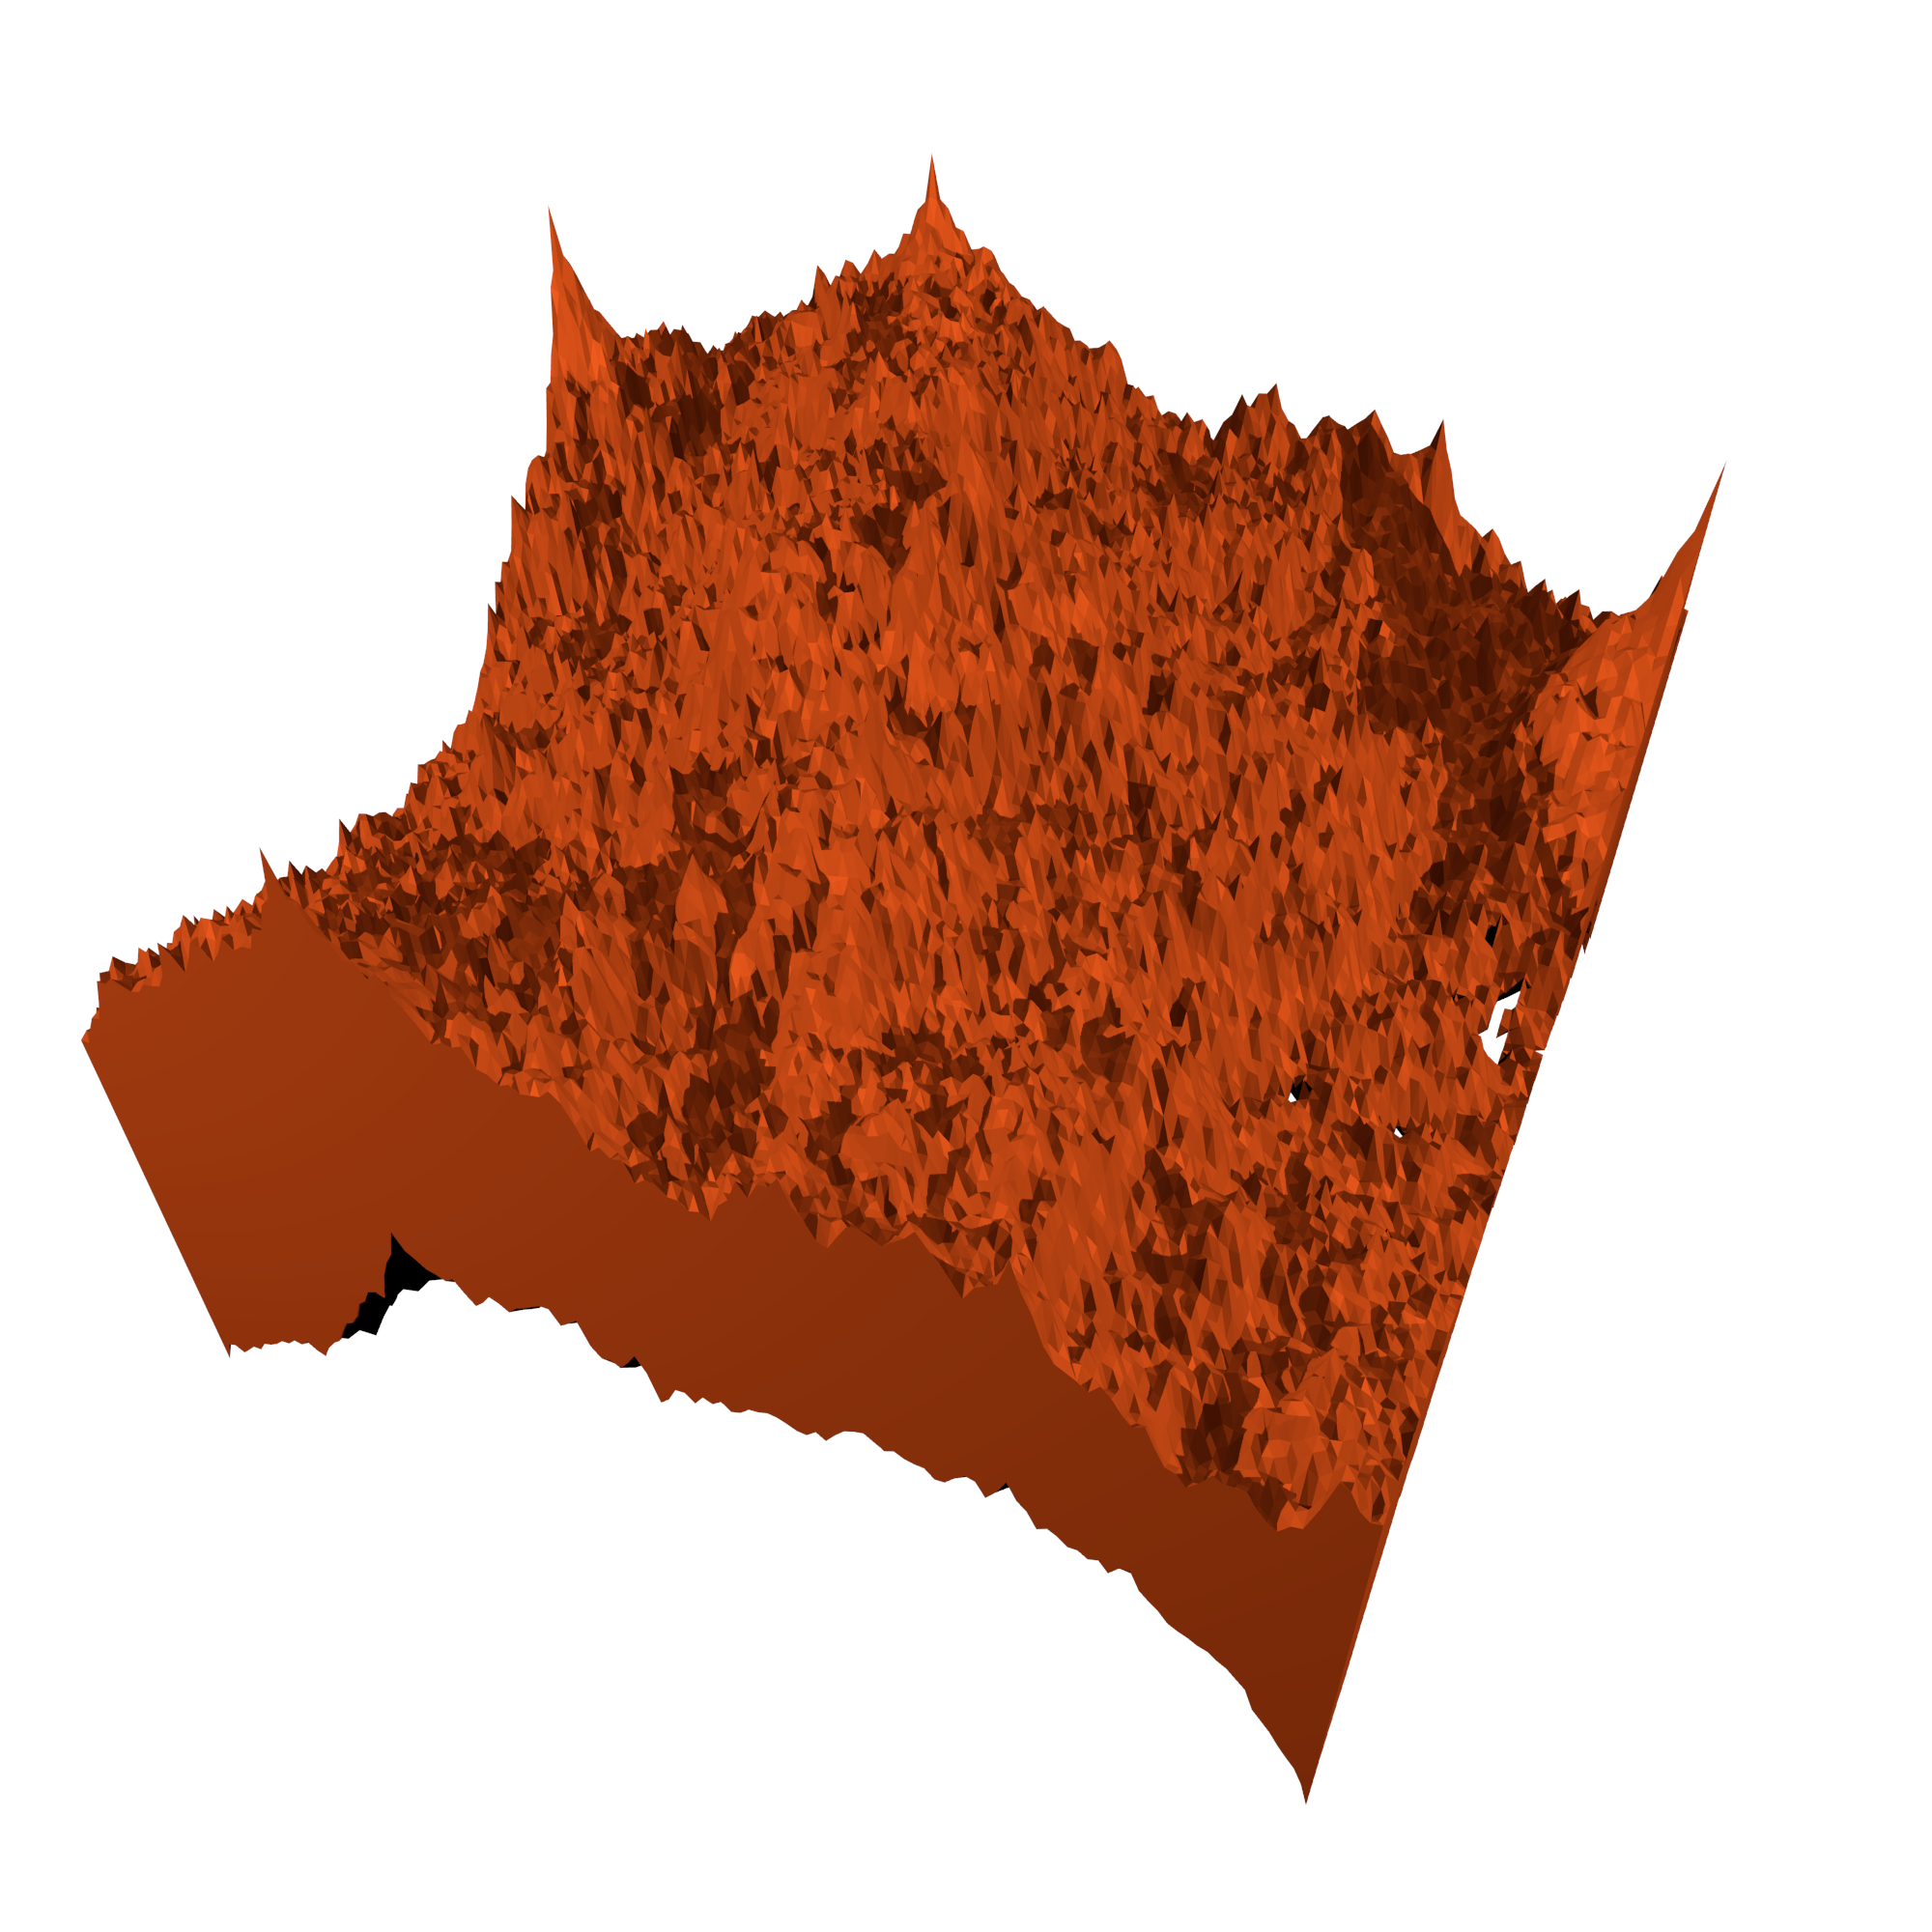
\includegraphics[width=0.6\textwidth]{images/fracture/fracture.png}
%     \caption{
%         A model of a fracture.
%         \label{fig:fracture_model}
%     }
% \end{figure}

\begin{figure}
    \centering
    \begin{subfigure}[b]{0.35\textwidth}
        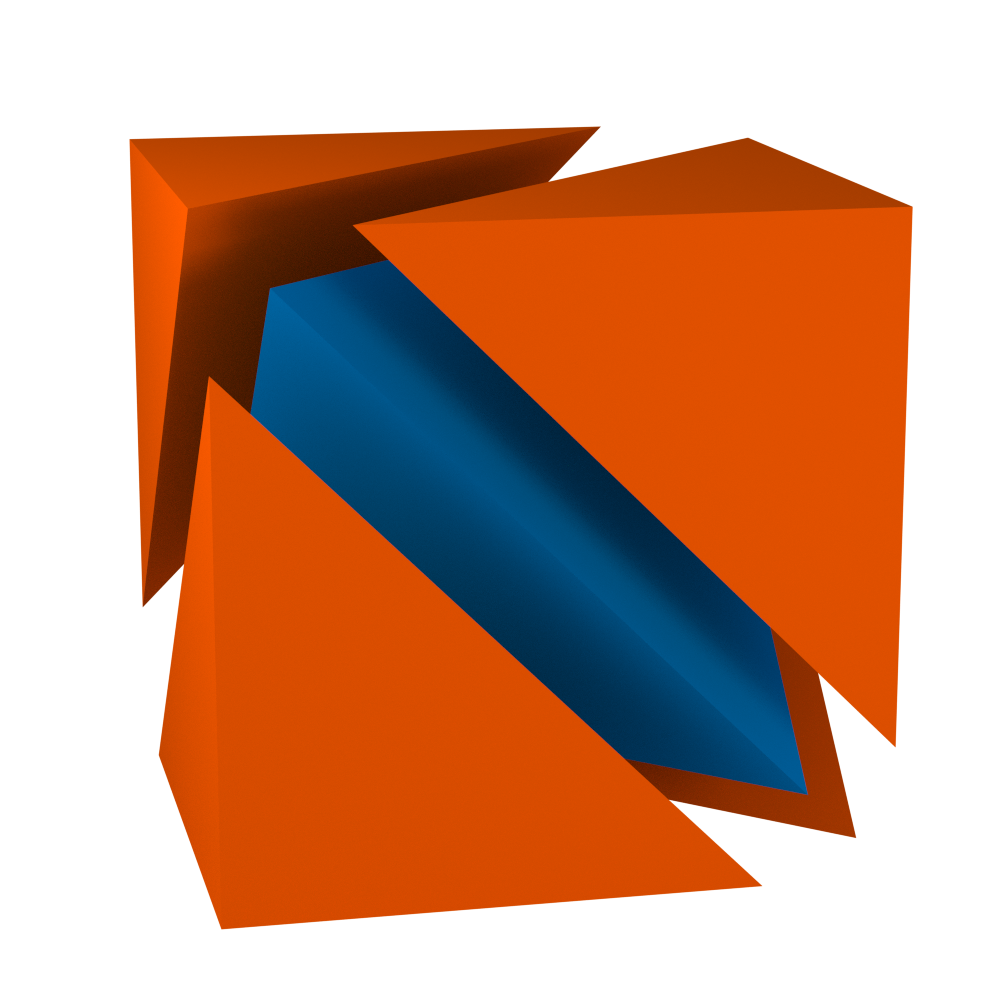
\includegraphics[width=\textwidth]{images/fracture/hexahedron_to_tetrahedra01_cycles_n200.png}
        \caption{Illustration of how to divide a convex hexahedron into five tetraheda.}
        \label{fig:hex_to_tetra}
    \end{subfigure}
    \hspace{5mm}
    \begin{subfigure}[b]{0.55\textwidth}
        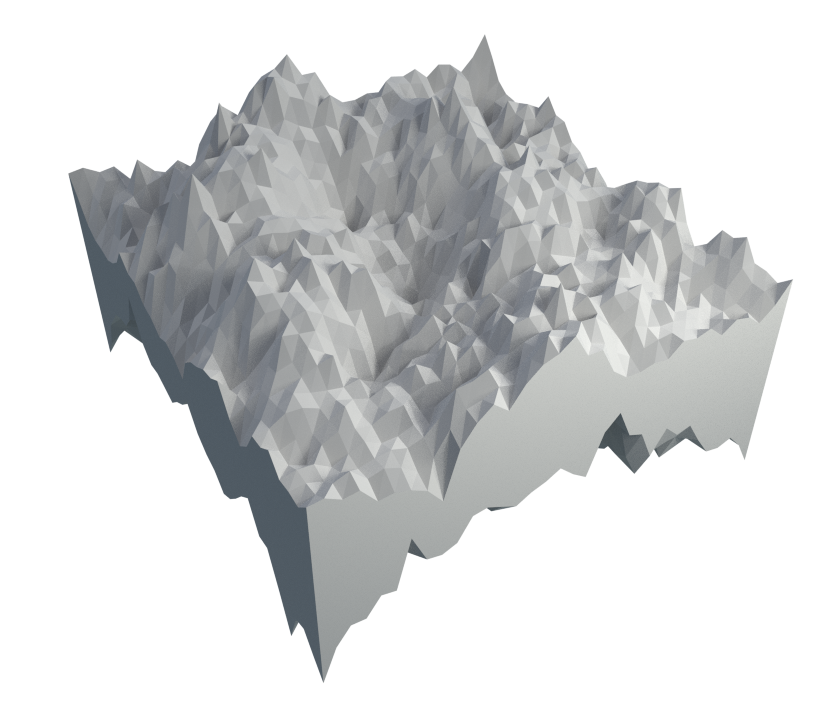
\includegraphics[width=\textwidth]{images/fracture/fracture05_n200.png}
%         \includegraphics[width=\textwidth]{images/fracture/large_fracture04_300dpi_w20cm}
        \caption{A random fracture made from two periodic heightmaps.}
        \label{fig:fracture_model}
    \end{subfigure}
\end{figure}

\subsubsection{Finding a point inside a tetrahedron}
% To calculate if a point is inside a tetrahedron we utilize the \emph{oriented} volume of a tetrahedron. The oriented volume of a tetrahedron with vertices $\bvec a$, $\bvec b$, $\bvec c$ and $\bvec d$ can be calculated as
% \begin{align*}
%     V = \frac{1}{6}(\bvec a - \bvec d)\big[(\bvec b - \bvec d)\times(\bvec c - \bvec d)\big].
% \end{align*}
% The \emph{ordered} volume simply means that the order of the vertices will determine the sign of the volume. The sign of the volume will be determined by on which side of the plane between $\bvec b$, $\bvec c$ and $\bvec d$ the point $\bvec a$ lies. The cross product $(\bvec b - \bvec d)\times(\bvec c - \bvec d)$ gives a normal vector to the plane, and the dot product projects $(\bvec a - \bvec d)$ onto this normal. The sign of the dot product is positive if $\bvec a$ is located the side of the plane which the normal points towards, and negative else.

% We then compare the sign of the volume of the tetrahedra to the signs of the volumes of four tetrahedra constructed by replacing one of the vertices of the tetrahedra with the point we want to find out if is inside the tetrahedra.



% A tetrahedron consists of four points 
% % $\bvec a$, $\bvec b$, $\bvec c$, and $\bvec d$, 
% % $\bvec r_i$ for $i\in\{1,2,3,4\}$,
% % $x$, $b$, $c$, and $d$, 
% $x_i$ for $i\in\{1,2,3,4\}$,
% and four faces spanned out by the four possible combinations of the four points. For a face spanned by the vectors $\bvec r_i = x_i - x_j$ and $\bvec r_j = x_k - x_j$, where, we can see if a point $P$ is on the same side of the face as the point $\bvec x_{l\neq i,j,k}$ not used to construct the face by doing some geometry. We calculate the normal vector to the face by the cross product $\bvec n = \bvec r_i\times\bvec r_j$. This gives us a normal vector $\bvec n$ to the surface. We then find the sign of dot products $\bvec n (P - x_j)$ and $\bvec n(x_l - x_j)$



A tetrahedron consists of four points $\bvec a$, $\bvec b$, $\bvec c$, and $\bvec d$ and four faces, spanned by the four possible combinations of the four points. For a face spanned by the points $\bvec a$, $\bvec b$, and $\bvec c$ we can find if a point $\bvec P$ is on the same side of the face as the point $\bvec d$ (the point not used to construct the face) by doing some geometry. We calculate the cross product 
\begin{align*}
    \bvec n = (\bvec a-\bvec c)(\bvec b-\bvec c),
\end{align*}
which gives us the normal vector to the surface $\bvec n$. We then find the sign of dot products 
\begin{align*}
    &\bvec n\cdot(\bvec P - \bvec c), \\
    &\bvec n\cdot(\bvec d - \bvec c).
\end{align*}
If the sign of these dot products is the same, we know that the point $\bvec P$ is on the same side of the face as the point $\bvec d$. We now see that if we do this for all four faces of the tetrahedra, we know that the point $\bvec P$ is inside the tetrahedra if the signs of all pairs of dot products are equal.



% Calculating wether a point is inside a tetrahedron can be reduced to comparing the sign of five different matrix determinants. If we have a point $P = (x,y,z)$ and the four vertices of the tetrahedron are $(x_i, y_i, z_i)$ for $i\in \{1,2,3,4\}$, we can find if the point is inside the tetrahedron by checking if the the following five matrix determinants have the same sign
% \begin{align*}
%     &\begin{vmatrix}
%         x_1 & y_1 & z_1 & 1 \\
%         x_2 & y_2 & z_2 & 1 \\
%         x_3 & y_3 & z_3 & 1 \\
%         x_4 & y_4 & z_4 & 1
%     \end{vmatrix},&
%     &\begin{vmatrix}
%         x & y & z & 1 \\
%         x_2 & y_2 & z_2 & 1 \\
%         x_3 & y_3 & z_3 & 1 \\
%         x_4 & y_4 & z_4 & 1
%     \end{vmatrix},&
%     &\begin{vmatrix}
%         x_1 & y_1 & z_1 & 1 \\
%         x & y & z & 1 \\
%         x_3 & y_3 & z_3 & 1 \\
%         x_4 & y_4 & z_4 & 1
%     \end{vmatrix},&
%     \\
% %     \vspace{5mm}
%     \\
%     &\begin{vmatrix}
%         x_1 & y_1 & z_1 & 1 \\
%         x_2 & y_2 & z_2 & 1 \\
%         x & y & z & 1 \\
%         x_4 & y_4 & z_4 & 1
%     \end{vmatrix},&
%     &\begin{vmatrix}
%         x_1 & y_1 & z_1 & 1 \\
%         x_2 & y_2 & z_2 & 1 \\
%         x_3 & y_3 & z_3 & 1 \\
%         x & y & z & 1
%     \end{vmatrix}.&
% \end{align*}

\chapter{Measurements}
\section{Voxelation, calculating distances, finding neighbors, neighbor lists, periodicity tricks\label{sec:voxelation}}
When doing calculations and measurements on a molecular system, we often need information about the neighboring atoms of each atom. Establishing which atoms are within a certain radius of each atom is not trivial; the trivial way of checking each atom against all other atoms scales as $\mathcal{O}(N^2)$, $N$ being the number of atoms. There are many clever algorithms for finding nearest neighbors, often called a ``nearest neighbor search'' (see \url{http://www.slac.stanford.edu/cgi-wrap/getdoc/slac-r-186.pdf} and references in that paper, especially ``11. Levinthal 1966''). Our problem is a very specific problem: to find all neighbors within a certain radius of a point, for all points. We didn't find any algorithms for solving this specific problem, and the usual algorithms can't benefit from the fact that we need to find the nearest neighbors of \emph{all} points.

Our solution to the problem is inspired by the ``cell list'' method used in MD integrators\hl{(see Frenkel Appendix F)}, and uses a method we call ``voxelation''/\emph{voxelation}. If we want to find all neighbors within a radius $dr$ we divide the system into 3-dimensional boxes (\emph{voxels}) of size $l = dr$. We then loop through all atoms, sorting each atom into the box it belongs in. To find the neighbors within the radius $dr$ of an atom at position $\rvec$ we now only have to find which box the atoms belongs to, and check the distance between the atom and all atoms in that box, and between and all atoms in the 26 neighboring boxes\todo{replace all ``box'' with ``voxel'' ?}. Pseudocode for this can be seen below \cref{list:voxels}

\todo[inline]{Distance between atoms, $r^2$ instead of $r$}

%     \begin{cppcode*}{gobble=8}
%         for (int i = 0; i < atoms.size(); i++)
%         {
%             int ix = floor(atoms[i].position().x() / voxelSize);
%             int iy = floor(atoms[i].position().y() / voxelSize);
%             int iz = floor(atoms[i].position().z() / voxelSize);
%             voxel[ix][iy][iz].push_back(i);
%         }
%     \end{cppcode*}
%     
%     \begin{cppcode*}{gobble=8}
%         // Loop over all atoms
%         for (int i = 0; i < atoms.size(); i++)
%         {
%             // Index of the voxel this atom belongs to
%             int i1 = floor(atoms[i].position().x() / voxelSize);
%             int j1 = floor(atoms[i].position().y() / voxelSize);
%             int k1 = floor(atoms[i].position().z() / voxelSize);
%             
%             // Loop over all 27 neighbor voxels (including self)
%             for (int di = -1; di <= 1; di++)
%             for (int dj = -1; dj <= 1; dj++)
%             for (int dk = -1; dk <= 1; dk++)
%             {{{
%                 // Find index of neighbor voxel using
%                 // periodic boundary conditions
%                 // nx, ny, nz is the number of voxels in each direction
%                 int i2 = (i1 + di + nx) % nx;
%                 int j2 = (j1 + dj + ny) % ny;
%                 int k2 = (k1 + dk + nz) % nz;
%                 
%                 // Loop over atoms in neighbor voxel
%                 for (j = 0; j < voxel[i2][j2][k2].size(); j++)
%                 {
%                     int k = voxel[i2][j2][k2][j];
%                     vec3 dr = atoms[k].position() - atoms[i].position();
%                     
%                     // Minimum image convention
%                     for (int dim = 0; dim < 3; dim++)
%                     {
%                         if      (dr[dim] >  L[dim]/2.0) dr[dim] -= L[dim];
%                         else if (dr[dim] < -L[dim]/2.0) dr[dim] += L[dim];
%                     }
%                     
%                     // Calculate dr^2 instead of sqrt(dr^2), since sqrt() is a very 
%                     // slow operation, and in this case is unnecessary
%                     double drSquared = dr.lengthSquared();
%                 }
%             }}}
%         }
%     \end{cppcode*}

\begin{listing}[H]
\begin{cppcode*}{gobble=4}
    for (Atom *atom : atoms)
    {
        // Index of the voxel this atom belongs to
        int i = floor(atom.position().x() / voxelSize);
        int j = floor(atom.position().y() / voxelSize);
        int k = floor(atom.position().z() / voxelSize);
        voxels[i][j][k].push_back(atom);
    }
\end{cppcode*}
\caption{A very long caption on this very interesting listing to see what happens when we get to the end of the line bla bla bla bla bla bla bla bla bla bla bla bla bla bla bla bla bla bla bla bla bla bla bla bla bla bla bla bla bla bla bla bla 
    \label{list:voxels}
}
\end{listing}

\begin{listing}[H]
\begin{cppcode*}{gobble=4}
    // Loop over all atoms
    for (Atom *atom1 : atoms)
    {
        // Index of the voxel this atom belongs to
        int i1 = floor(atom1.position().x() / voxelSize);
        int j1 = floor(atom1.position().y() / voxelSize);
        int k1 = floor(atom1.position().z() / voxelSize);
        
        // Loop over all 27 neighbor voxels (including self)
        for (int di = -1; di <= 1; di++)
        for (int dj = -1; dj <= 1; dj++)
        for (int dk = -1; dk <= 1; dk++)
        {{{
            // Index of neighbor voxel using periodic boundary conditions
            // nx, ny, nz is the number of voxels in each direction
            int i2 = (i1 + di + nx) % nx;
            int j2 = (j1 + dj + ny) % ny;
            int k2 = (k1 + dk + nz) % nz;
            
            // Loop over atoms in neighbor voxel
            for (Atom *atom2 : voxels[i2][j2][k2])
            {
                if (atom2 != atom1)
                {
                    double drSquared = 
                        calculateDistanceSquaredBetweenAtoms(atom1, atom2);
                }
            }
        }}}
    }
    
\end{cppcode*}
\caption{Test
    \label{list:neighbors}
}
\end{listing}

\begin{listing}[H]
\begin{cppcode*}{gobble=4}
    calculateDistanceSquaredBetweenAtoms(Atom *atom1, Atom atom2)
    {
        vec3 dr = atom2.position() - atom1.position();
        
        // Minimum image convention
        for (int dim = 0; dim < 3; dim++)
        {
            if      (dr[dim] >  L[dim]/2.0) dr[dim] -= L[dim];
            else if (dr[dim] < -L[dim]/2.0) dr[dim] += L[dim];
        }
        
        // Calculate dr^2 instead of sqrt(dr^2), since sqrt() is a very 
        // slow operation, and in this case is unnecessary
        double drSquared = dr.lengthSquared();
    }
\end{cppcode*}
\caption{Test
    \label{list:dr2}
}
\end{listing}

\section{Mean square displacement}
    
\section{Density}
\section{Distance to atom}
We developed a program that finds the distance to the nearest atom, in all points of the 
\begin{figure}[h!]
    \centering
    \includesvg[width=1.0\textwidth, svgpath = ./images/distance_to_atom/]{SiO2_06_slice_r05_n256}
    \caption{$r = 5$ \Ang}
    \label{fig:distance_to_atom_r05}
\end{figure}

\begin{figure}[h!]
    \centering
    \includesvg[width=1.0\textwidth, svgpath = ./images/distance_to_atom/]{SiO2_06_slice_r20_n256}
    \caption{$r = 20$ \Ang}
    \label{fig:distance_to_atom_r20}
\end{figure}

\section{``Generation matrix''}
    Not very useful. Much of the same as distance to atom, only worse (but faster).
\section{``Voxel counter''}
    A histogram of the fraction of voxels that has one or more atom in them vs. the voxel size in x-, y-, and z-direction.
\section{Cage cage correlation}
\section{Tetrahedral order parameter}
\section{Surface area of pores}

\part{Results}
    \section{Mean square displacement}
    \section{Distance to atom}
    \section{Area}
    \section{Volume?}

\part{Discussion}

\part{Appendices}

\printbibliography
% \bibliography{JabRef_database,Mendeley_database}

\end{document}
